\documentclass[11pt,reqno,final]{amsart}

\pdfcompresslevel=0
\pdfobjcompresslevel=0

\usepackage[dvipsnames]{xcolor}% adds colors
\usepackage{amsmath, amsthm}% {amsfonts, amssymb}

% New Characters
\usepackage[latin1]{inputenc}%
\usepackage[T1]{fontenc}

\usepackage{MnSymbol}
\usepackage[normalem]{ulem}% underlining

\usepackage[theoremfont, largesc]{newpxtext} % different text,math font
\usepackage{newpxmath}

\makeatletter
\DeclareMathRadical{\sqrtsign}{symbols}{112}{largesymbols}{112}
% \let\sqrt=\undefined
% \DeclareRobustCommand\sqrt{\@ifnextchar[\@sqrt{\mathpalette\@x@sqrt}]}
% \def\@x@sqrt#1#2{%
%  \setbox\z@\hbox{$\m@th#1\sqrtsign{\mkern1mu #2}$}
%  \mkern3mu\box\z@}
\makeatother




% Page Typesetting
\usepackage[final]{microtype}
\usepackage{relsize}
\usepackage[margin=1in]{geometry}
\usepackage{framed}
\usepackage{tikz}
\usepackage{setspace}

\usepackage{hyperref}
\hypersetup{
  final,
  pdftitle={Math 135 - Project 1},
  pdfauthor={Bonventre}, 
  linktoc=page,
  pagebackref,
  colorlinks=true,
  citecolor=PineGreen,
  linkcolor=PineGreen,
  linkbordercolor=PineGreen,
}


% Internal References

\usepackage[inline,shortlabels]{enumitem}

\numberwithin{equation}{section} 
\numberwithin{figure}{section}

\usepackage[nameinlink,capitalise,noabbrev]{cleveref}

\crefname{equation}{}{} % get \cref to behave as \eqref

% \theoremstyle{plain} % bold name, italic text
\newtheorem{theorem}[equation]{Theorem}%
\newtheorem*{theorem*}{Theorem}%
\newtheorem{lemma}[equation]{Lemma}%
\newtheorem{proposition}[equation]{Proposition}%
\newtheorem{corollary}[equation]{Corollary}%
\newtheorem{conjecture}[equation]{Conjecture}%
\newtheorem*{conjecture*}{Conjecture}%
\newtheorem{claim}[equation]{Claim}%
\newtheorem{question}{Question}

\theoremstyle{definition} % bold name, plain text
\newtheorem{definition}[equation]{Definition}%
\newtheorem*{definition*}{Definition}%
\newtheorem{example}[equation]{Example}%
\newtheorem*{example*}{Example}%
\newtheorem{remark}[equation]{Remark}%
\newtheorem{notation}[equation]{Notation}%
\newtheorem{convention}[equation]{Convention}%
\newtheorem{assumption}[equation]{Assumption}%
\newtheorem{exercise}[question]{Exercise}

% ---------- macros
\newcommand{\set}[1]{\left\{#1\right\}}%
\newcommand{\sets}[2]{\left\{ #1 \;|\; #2\right\}}%
\newcommand{\longto}{\longrightarrow}%
\newcommand{\into}{\hookrightarrow}%
\newcommand{\onto}{\twoheadrightarrow}%

\usepackage{harpoon}
\newcommand{\vect}[1]{\text{\overrightharp{\ensuremath{#1}}}}

\newcommand{\del}{\partial}%

\newcommand{\ki}{\chi}
\newcommand{\ksi}{\xi}
\newcommand{\Ksi}{\Xi}

\newcommand{\dlim}{\displaystyle\lim}

% %%%%%%%%%%%%%%%%%%%%%%%%%%%%%%%%%%%%%%%%%%%%%%%%%%%%%%%%%%%%%%%%%%%%%%%%%%%%%%%%%%%%%%%%%%%%%%%%%%%%

\begin{document}
\onehalfspacing

\begin{center}
        \textbf{\Large Math 135, Calculus 1, Fall 2020}\\[10pt]
        {\large Project 1: Modeling an epidemic.}\\
        Due: \textbf{Friday, October 2} by 11:59pm.
\end{center}

\thispagestyle{empty}

\renewcommand{\thesection}{\Alph{section}}

\subsection*{The Project:}
You will be building and evaluating different functions modeling the \textit{cumultative number of cases of COVID-19} in New York City between March 1 and May 30.


\subsection*{Components}

This project has two components: a spreadsheet and a written report.
Accordingly, the questions below have two components:

First, each group has a prepared Google Sheets document.
Every problem but the last requires you to work in this spreadsheet, either by graphing or making calculations.
This worksheet will be included as part of your project.
You may add to or modify this spreadsheet, if needed, as you wish to solve the problems and present your solutions.

Second, each group will need to prepare a written report, clearly written in complete sentences.
Each problem includes a set of ``discussion questions''.
As you are addressing each problem, keep these questions in mind, and in your report, please reflect and answer these questions.


\subsection*{Setup}
When modeling epidemics, an important variable is the \textit{basic reproduction number} $R_0$.
The basic reproduction number is the expected (or average) number of new cases generated by a single infected individual.
This (positive) number is effected by many factors, including
biological conditions of the pathogen, environmental conditions, and the behavior of the infected population, 

Throughout this project, we make the following assumptions:
\begin{enumerate}[(i)]
\item Each infected individual infects $R_0$-many new individuals over the course of \textbf{one week} (the approximate time duration an infected person is contageous).
\item $R_0$ is constant over each time period in consideration.
\end{enumerate}

\newpage

\section*{Part A: Building a simple model using $R_0$}

Your first set of problems involve building a simple model for the spread of a disease based on
the initial population $Q_0$ and a constant basic reproduction number $R_0$.

\begin{enumerate}[(1)]\itemsep+20pt
\item Suppose we have an initial infected population of 1000 people.
        Compute the total infected population, weekly, for 10 weeks, for the following values of $R_0$: 0.5, 1, 2, 4.
        Present this data graphically in \textcolor{yellow}{Sheet One} of your project's Google Spreadsheet.\\

        Discussion questions:
        \begin{itemize}
        \item Is the total infected population function increasing, decreasing, or neither, as a function of time?
        \item How did you compute these values?
        \end{itemize}
        
        
\item This type of \textit{unrestricted growth} can be modeled using an exponential function $f(x) = A \cdot b^x$.
        Find a general function $Q(t)$ which models the total infected population as a function of time $t$ (in weeks),
        with initial population $Q_0$ and basic reproduction number $R_0$.
        Graph two particular examples in \textcolor{yellow}{Sheet One} using the values from Question (1).\\

        Discussion questions:
        \begin{itemize}
        \item Your graph from Part A(1) is individual points, while this graph from Part A(2) is continuous. How might this be a reflection in real-world reporting of pandemics?
        \item What are the indepedent and dependent variables of your function?
        \end{itemize}
        
\item Modify your equation $Q(t)$ so the input is in terms of \textbf{days} $d$ as opposed to weeks.\\

        Discussion questions:
        \begin{itemize}
        \item Which do you expect to be more accurate: the daily counts or weekly counts from this model?
        \end{itemize}
        
\end{enumerate}

\newpage
\section*{Part B: Using your model}

You will use your equation $Q(d)$ from Part 1 above to model the spread of COVID-19 in New York in March and April.
Throughout, we will be using a funciton $f(d)$ which represents the total number of confirmed COVID-19 cases ffrom the beginning of March to the end of day $d$.


\textcolor{blue}{Sheet Two} contains the data and a chart of the total number of reported cases of COVID-19 in New York between \textcolor{blue}{March 1 and March 20}.

\begin{enumerate}[(1)]\setcounter{enumi}{3}\itemsep+20pt
\item  Use your general equation to create a model $Q_1(d)$ for the total COVID-19 cases in New York from \textcolor{blue}{March 1 through March 20}.
        That is, choose values of $R_0$ and $Q_0$ that you decide best fits this data.
        Add a graph of your model $Q_1(d)$ to the chart in \textcolor{blue}{Sheet Two}.\footnote{To add a function to a chart, right click on the chart, select ``Data range'', click ``add series'', tap the 4-squares icon, and select your range of values in the spreadsheet.}\\        
        
        Discussion questions:
        \begin{itemize}
        \item What date does $d=0$ correspond to? What is the domain of your function?
        \item Translate the equation $f(10) = 175$ into an explanatory English sentence. Do the same for your value of $Q_1(10)$.
        \item What are different factors you considered when evaluating different possible choices of $R_0$ and $Q_0$?
        \item How well does the \textit{mathematical model} $Q_1(d)$ represent the \textit{actual} infection count $f(d)$?
                What are some real-world explainations which may account for this?
        \end{itemize}
\end{enumerate}


$ $

New York City went into full lockdown on March 20. You will now investigate how the data changes after this point.
\textcolor{red}{Sheet Three} contains the data and a chart for \textcolor{red}{March 20 through April 30}.

\begin{enumerate}[(1)]\setcounter{enumi}{4}\itemsep+20pt
\item Use your equation $Q_1(d)$ to model the total COVID-19 cases in New York from \textcolor{red}{March 20 through April 30.}
        That is, using the same $R_0$ value as in Part B(1) and taking $Q_0 = Q_1(20)$,
        add a graph of your model to the chart in \textcolor{red}{Sheet Three} containing the real world data.\\
        
        Discussion questions:
        \begin{itemize}
        \item What date does $d=0$ now correspond to?
        \item How well does $Q_1(d)$ model the spread of COVID-19 in late March and April? What does $Q_1(d)$ predict? (Note that the population of New York City is about 8.3 million.)
        \item Does the real data qualitatively change after March 20?
        \item Use the above modeling to conclude whether or not the lockdown was effective in preventing the spread of COVID-19.
        \end{itemize}

\item Build a new function $Q_2(d)$ to model the spread of COVID-19 between \textcolor{red}{March 20 and April 30};
        that is, choose new values of $R_0$ and $Q_0$ for a new model $Q_2(d)$ to fit the data from March 20 through April 30.
        Graph your model $Q_2(d)$  
        on the same set of axes in \textcolor{red}{Sheet Three} as in Part B(2).\\
        
        Discussion questions:
        \begin{itemize}
        \item How does $Q_0$ for $Q_1(d)$ compare with $Q_0$ for $Q_2(d)$?
        \item How does $R_0$ for $Q_1(d)$ compare to $R_0$ of $Q_2(d)$? What are some real-world reasons that might be the case?
        \item How well does $Q_2(d)$ model the data from March 20 through April 30? What can we conclude about the basic reproduction number over this time period?
        \end{itemize}
        
\item Use a \textit{line} to model the spread of COVID-19 between \textcolor{red}{March 20 and April 30}.
        That is, decide on values of $m$ and $b$ so that the function $L(d) = md+b$ best fits this data.
        Graph this model on the same set of axes in \textcolor{red}{Sheet Three} as in Part B(2) and B(3).\\
        
        Discussion questions:
        \begin{itemize}
        \item How did you evaluate your choices of $m$ and $b$?
        \item How many cases does your linear model predict for March 20? How does this compare with the real data? Does this bother you? Why or why not?
        \item Which of $Q_2(d)$ or $L(d)$ better models the spread of COVID-19 over this time period ? Why might this be?
        \item Linear growth is not unrestricted. What are some scenarios which are better modeled by linear growth?
        \end{itemize}
\end{enumerate}

\newpage
\section*{Part C: Logistic Growth}

Epidemics are often accurately modeled by a family of functions with ``S''-shaped graphs called \textbf{logistic curves}:
\[
        S(d) = \dfrac{\theta_1}{1 + e^{-\theta_2 \cdot (t - \theta_3)}}
\]
\begin{minipage}{.5\textwidth}
        \begin{center}
                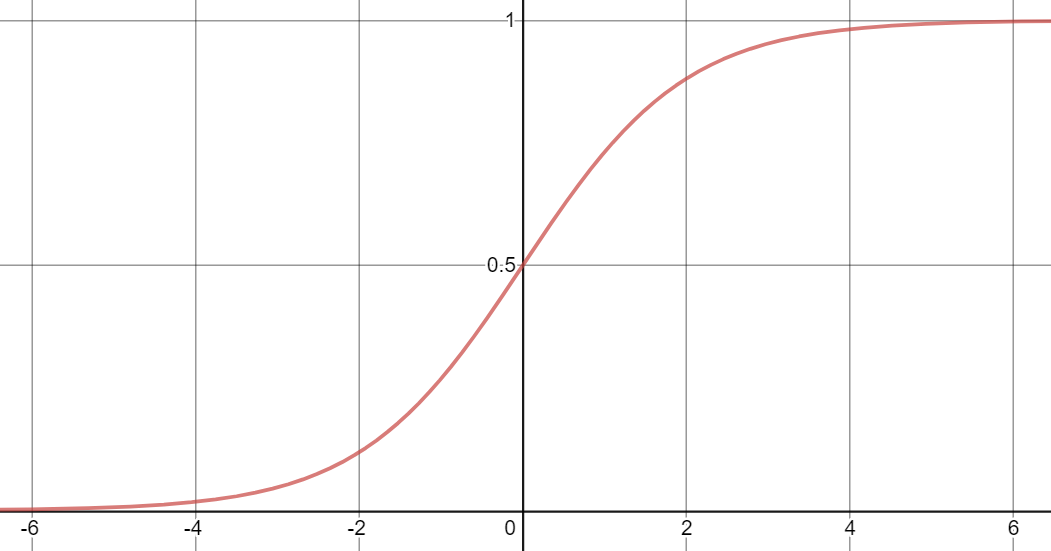
\includegraphics[width=3in]{logistic}
        \end{center}
\end{minipage}
\begin{minipage}{.5\textwidth}
        \begin{center}
                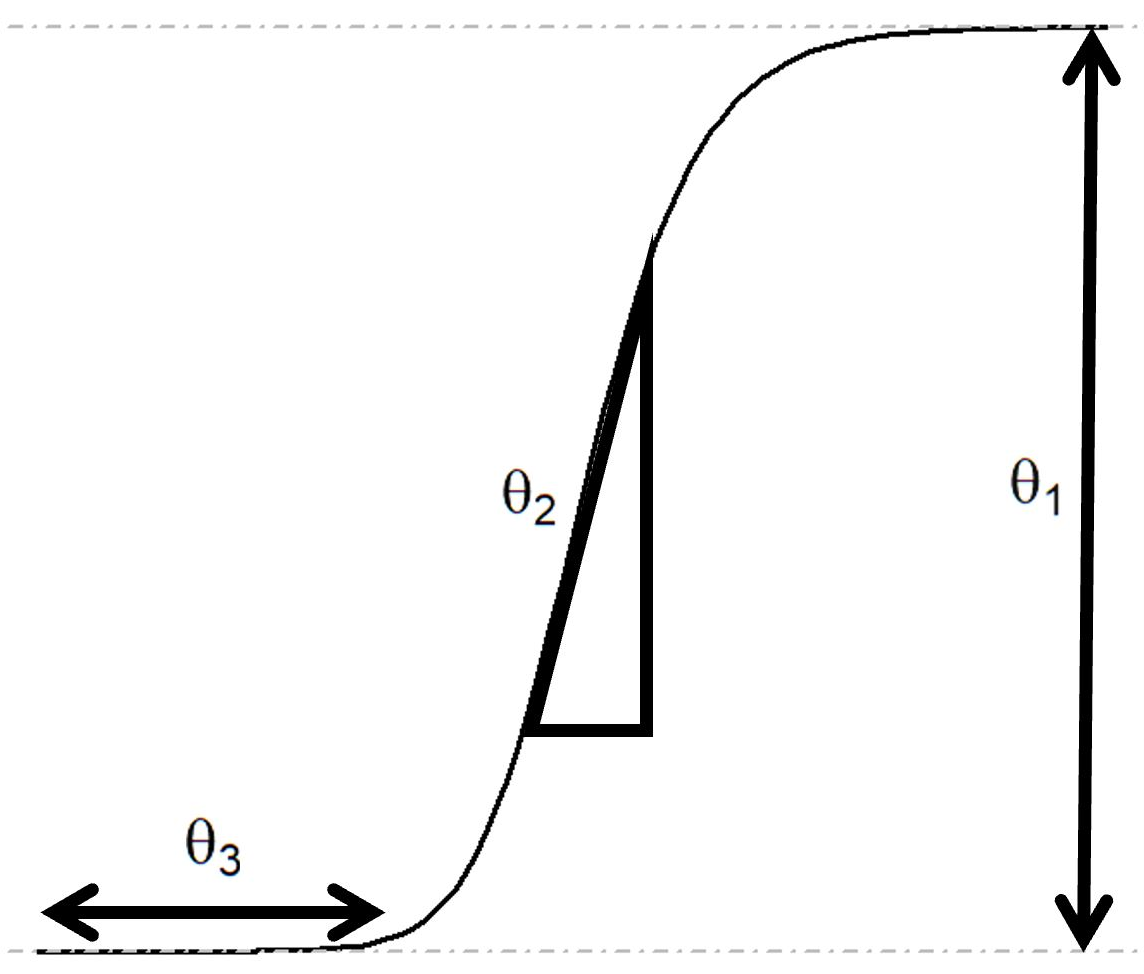
\includegraphics[width=2in]{logparams}
        \end{center}
\end{minipage}

A logistic model has been built into \textcolor{OliveGreen}{Sheet Four}, along with a graph of real-world data from \textcolor{OliveGreen}{March 1 through May 30}.
\begin{enumerate}
\item[(8)] Build a logistic model to fit this data.
        That is, choose values for the parameters $\theta_1$, $\theta_2$, and $\theta_3$ that you decide best fit this data.\\
        
        Discussion questions:
        \begin{itemize}
        \item Why is an ``S''-shaped curve more appropriate for an epidemic? What real-world actions may have an influence on the shape of the curve of total infected?
        \item What are some difference between your logistic model $S(d)$ and the real data? What might account for this discrepency?
        \item What is the long-term behavior of your model? That is, what is the limit $\dlim_{t \to \infty}S(t)$? What does this represent? How does this number compare to the 8.3 million total population in New York City?
        \end{itemize}
\end{enumerate}

$ $

\section*{Part D: Reflection}

\begin{enumerate}
\item[(9)] Discuss one thing your group has learned during this project.
\end{enumerate}


\end{document}
